\chapter{Affichage des tentacules en arc de cercle}
\begin{figure}[!ht]
    \centering
    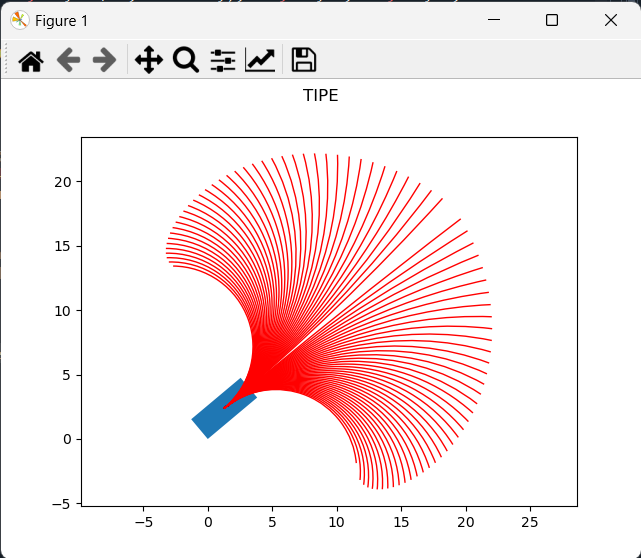
\includegraphics[scale=0.7]{Affichage arcs de cercle.png}
\end{figure}
\vspace{120pt}

\begin{mintedbox}{python}
"""
Affiche la voiture avec ses tentacules en forme d'arcs de cercle.
"""


class Tentacule:
    def __init__(self, voiture, k, delta_k, axes):
        self.axes = axes

        self.L1 = 8 + 72 * (voiture.vitesse/voiture.vitesse_max)**1.2  # formule empirique, équation (9.5) p.123
        # formules pour la longueur p.123 équation (9.4)
        # formules pour le rayon de courbure p.122 équation (9.3)

        if 1 <= k <= 40:  # tentacule à orienter vers la droite
            self.longueur = self.L1 + 20 * np.sqrt((k-1) / 40)
            self.courbure = -np.tan(delta_k) / voiture.longueur

            self.rayon = 1 / self.courbure
            self.angle_rad = self.longueur / self.rayon
            self.angle = self.angle_rad * 180 / np.pi

            self.patch = matplotlib.patches.Arc((voiture.x + self.rayon / 2, voiture.y), self.rayon, self.rayon, theta1=180 - self.angle, theta2=180, color='r')

        elif k == 41:
            self.longueur = self.L1 + 20 * np.sqrt((k-1) / 40)
            self.courbure = 0

            self.patch = matplotlib.patches.Arc((0, 0), 0, 0)

        else:  # 42<=k<=81   # tentacule à orienter vers la gauche
            self.longueur = self.L1 + 20 * np.sqrt((81-k) / 40)
            self.courbure = np.tan(delta_k) / voiture.longueur

            self.rayon = 1 / self.courbure
            self.angle_rad = self.longueur / self.rayon  # en radian
            self.angle = self.angle_rad * 180 / np.pi  # en degrés

            self.patch = matplotlib.patches.Arc((voiture.x - self.rayon / 2, voiture.y), self.rayon, self.rayon, theta1=0, theta2=self.angle, color='r')

        self.patch.set_transform( matplotlib.transforms.Affine2D().rotate_deg_around(voiture.x, voiture.y, voiture.angle - 90) + self.axes.transData)


class Voiture:
    def __init__(self, shape_voiture, x, y, axes):
        self.axes = axes
        self.longueur = LONGUEUR_VEHIC
        self.largeur = LARGEUR_VEHIC
        self.vitesse_max = VITESSE_MAX_VOIT
        self.accel_lat_max = ACCEL_LAT_MAX
        self.shape_voiture = shape_voiture

        self.vitesse = VITESSE_INIT_VOIT
        self.x, self.y = self.shape_voiture.get_center()
        self.angle = INCLINAISON_VOITURE_INIT

        self.courbure_max = self.accel_lat_max / self.vitesse ** 2  # formule p.122 équation (9.1)
        self.braquage_max = np.arctan(self.longueur * self.courbure_max)  # formule p.122 équation (9.2)

        self.transfo_init = self.shape_voiture.get_transform() + matplotlib.transforms.Affine2D().rotate_deg(90)


figure_ref_terre, axes_ref_terre = plt.subplots()
figure_ref_terre.suptitle("TIPE")
simulation_voision_terrestre = Simulation_Ref_Terre()

shape_voiture = matplotlib.patches.Rectangle(POSITION_VOITURE_INIT, LONGUEUR_VEHIC, LARGEUR_VEHIC, INCLINAISON_VOITURE_INIT)
voiture = Voiture(shape_voiture, 0, 0, axes_ref_terre)
axes_ref_terre.add_patch(voiture.shape_voiture)
tentacules = []
deltas = np.linspace(-voiture.braquage_max, voiture.braquage_max, 80)
for k in range(1, 81):
    tentacules.append(Tentacule(voiture, k, deltas[k-1], axes_ref_terre))
for k in range(80):
    axes_ref_terre.add_patch(tentacules[k].patch)


plt.autoscale()
plt.axis('equal')
plt.show()

\end{mintedbox}